\chapter{RH Agent Integration}
\minitoc
\clearpage
\section{Introduction}
This chapter presents Sprint 6, focused on integrating the RH Agent in the final stage of the project. The goal was simple: help HR users through a conversational assistant that can answer questions, guide them, and also query data when needed.

\section{Sprint Backlog}
For Sprint 6, the backlog focused on getting the RH Agent ready in a safe and usable way.
\begin{table}[H]
\centering
\renewcommand{\arraystretch}{1.2}
\begin{tabular}{|l|>{\raggedright\arraybackslash}p{10.2cm}|l|}
\hline
\textbf{ID} & \textbf{Backlog Item} & \textbf{Priority} \\
\hline
S6-BL-01 & Integrate RH Agent capabilities into the platform workflow. & High \\
\hline
S6-BL-02 & Connect RH Agent interactions to authorized backend endpoints. & High \\
\hline
S6-BL-03 & Validate response consistency and role-aware usage boundaries. & Medium \\
\hline
S6-BL-04 & Execute final stabilization and end-to-end verification. & Medium \\
\hline
\end{tabular}
\caption{Sprint 6 backlog}
\label{tab:sprint-6-backlog}
{\footnotesize\textit{Source: Author's work.}}
\end{table}

\section{Sprint Design}
The RH Agent was designed to be practical in real HR usage: clear replies, relevant context, and stable behavior during day-to-day operations.

\subsection{Conversation and interaction design}
We first designed interaction flows for the most common HR cases: asking about attendance, checking follow-up actions, and helping users move to the right page quickly. We also kept responses short and useful instead of overly verbose.

\Needspace{0.78\textheight}
\subsection{LangGraph routing design}
The RH Agent was built using \textbf{LangGraph} and \textbf{LangChain}, with \textbf{SQLAlchemy} for database access. The first thing the agent does is classify user input into two paths: a \textbf{chat} path and a \textbf{database-query} path. If the request is simple conversation, the agent replies directly. If it needs data, it goes through schema inspection, SQL generation, validation, execution, and finally response generation, with error handling at each important step.

Figure~\ref{fig:rh-agent-flow} summarizes the graph: input classification, chat node, database-query pipeline, and terminal success/error transitions.

\begin{figure}[H]
\centering
\IfFileExists{assets/rh/rh-agent-flow.jpg}{%
    \includegraphics[width=0.94\textwidth,height=0.58\textheight,keepaspectratio]{assets/rh/rh-agent-flow.jpg}
    }{%
        \fbox{\parbox{0.9\textwidth}{
            \centering
                \vspace{1.8cm}
                    \textit{Missing file: assets/rh/rh-agent-flow.jpg}\\
                        \textit{Insert RH Agent flow diagram (intent classification -> chat route / database route with SQL steps and error handling).}
                            \vspace{1.8cm}
                                }}
                                }
\caption{RH Agent flow with intent classification and SQL routing}
\label{fig:rh-agent-flow}
                                \end{figure}


                                \Needspace{0.90\textheight}
                                \section{Conception}
                                \Needspace{0.92\textheight}
                                \subsection{RH Agent sequence diagram}
                                The sequence diagram shows the full journey from user request to final response: user interaction, intent classification, graph routing, SQL access when needed, and streamed output.
                                Figure~\ref{fig:rh-agent-sequence-diagram} summarizes request routing, query lifecycle, response streaming, and interruption handling through the stop action.
                                \clearpage
                                \begin{figure}[p]
                                \centering
                                \vspace*{\fill}
                                \IfFileExists{diagrams/rh-agent/rh-agent-sequence-diagram.png}{%
                                    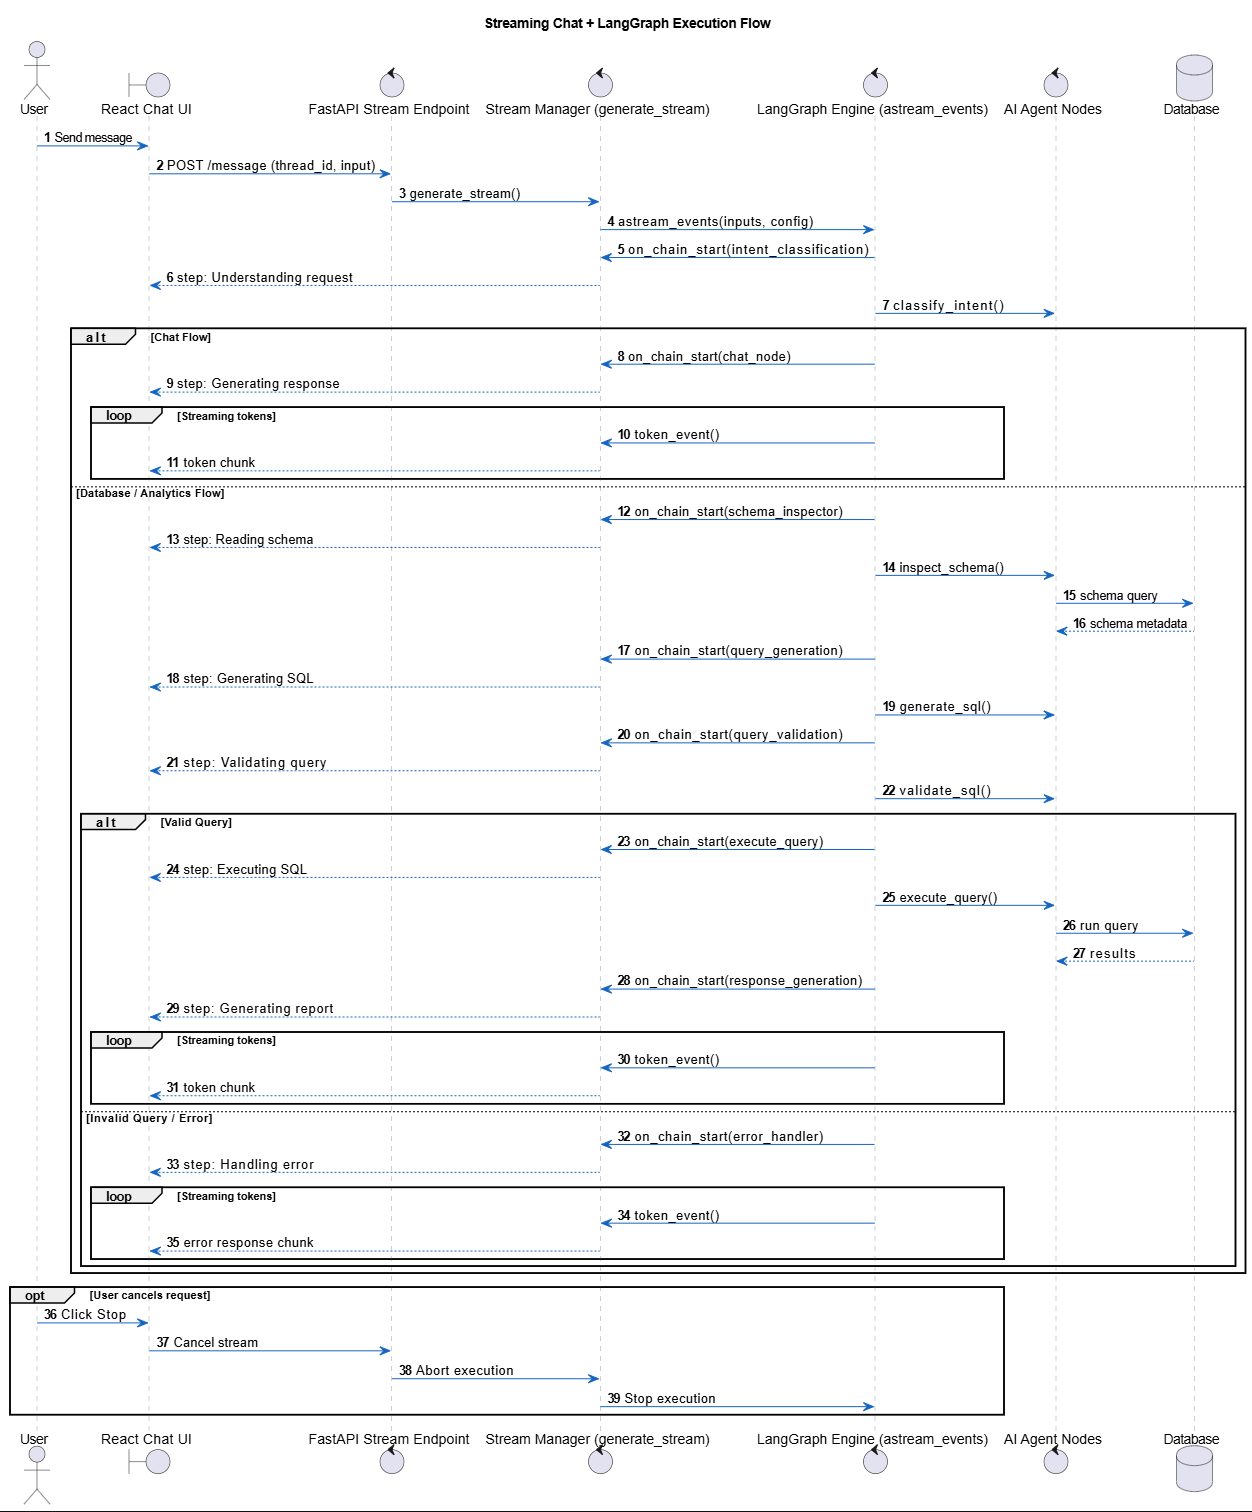
\includegraphics[width=\textwidth,height=0.88\textheight,keepaspectratio]{diagrams/rh-agent/rh-agent-sequence-diagram.png}
                                    }{%
                                        \fbox{\parbox{0.9\textwidth}{
                                            \centering
                                                \vspace{2.0cm}
                                                    \textit{Missing file: diagrams/rh-agent/rh-agent-sequence-diagram.png}\\
                                                        \textit{Insert RH Agent sequence diagram.}
                                                            \vspace{2.0cm}
                                                                }}
                                                                }
                                \caption{Sequence diagram of the RH Agent workflow}
                                \label{fig:rh-agent-sequence-diagram}
                                \vspace*{\fill}
                                \end{figure}
                                \clearpage



                                                                \Needspace{0.42\textheight}
                                                                \subsection{Agent state model conception}
                                                                In LangGraph, the \textbf{agent state} is the shared memory used by all nodes while a request is being processed. You can see it as one object that moves across the flow and keeps the key information needed at each step. We designed it to support both normal chat answers and database-query answers.

                                                                The state contains:
                                                                \begin{itemize}[noitemsep]
                                                                    \item \texttt{db\_context: str}: short database context (schema/table information) used to help the LLM generate relevant SQL.
                                                                        \item \texttt{messages: list[BaseMessage]}: conversation history between the user and the assistant.
                                                                            \item \texttt{user\_input: str}: the latest user message to process.
                                                                                \item \texttt{intent: Optional[str]}: detected route, typically \texttt{chat} or \texttt{database-query}.
                                                                                    \item \texttt{sql\_query: Optional[str]}: SQL generated by the query node before execution.
                                                                                        \item \texttt{sql\_is\_safe: bool}: safety flag showing whether the SQL passed validation checks.
                                                                                            \item \texttt{query\_result: str}: formatted database output returned to the user.
                                                                                                \item \texttt{error: Optional[str]}: error message captured when validation or execution fails.
                                                                                                \end{itemize}

                                                                                                For a bachelor-project perspective, this design is important because it separates responsibilities clearly: classification, SQL generation, validation, execution, and response formatting. Each step reads and updates only the fields it needs. This makes the agent easier to debug, safer for database access, and easier to maintain as new features are added.

                                                                                                \Needspace{0.28\textheight}
                                                                                                \section{Sprint Realization}
                                                                                                \subsection{Implementation outcomes}
                                                                                                \begin{itemize}[noitemsep]
                                                                                                    \item Integrated RH Agent module into the platform workflow.
                                                                                                        \item Connected RH Agent requests to selected backend services using LangChain and SQLAlchemy.
                                                                                                            \item Implemented intent classification to route requests between chat and database-query paths.
                                                                                                                \item Implemented schema inspection, SQL generation, query safety validation, execution, and error handling in the database route.
                                                                                                                    \item Implemented streaming response delivery so users can read the agent output progressively during generation.
                                                                                                                        \item Implemented a \textbf{Stop} control that allows users to interrupt generation in the middle of a conversation.
                                                                                                                            \item Integrated support for local LLM execution (Ollama) with compatibility for cloud-hosted models.
                                                                                                                                \item Performed stabilization and end-to-end verification.
                                                                                                                                \end{itemize}

                                                                                                                                \Needspace{0.72\textheight}
                                                                                                                                \subsection{RH Agent interface}
                                                                                                                                Figure~\ref{fig:rh-agent-interface} presents the integrated assistant interface and a sample guided interaction flow. It highlights how users can type natural requests, receive streamed responses, and interrupt generation when needed.

                                                                                                                                \begin{figure}[H]
                                                                                                                                \centering
                                                                                                                                \IfFileExists{assets/rh-agent/rh-agent-interface.jpg}{%
                                                                                                                                    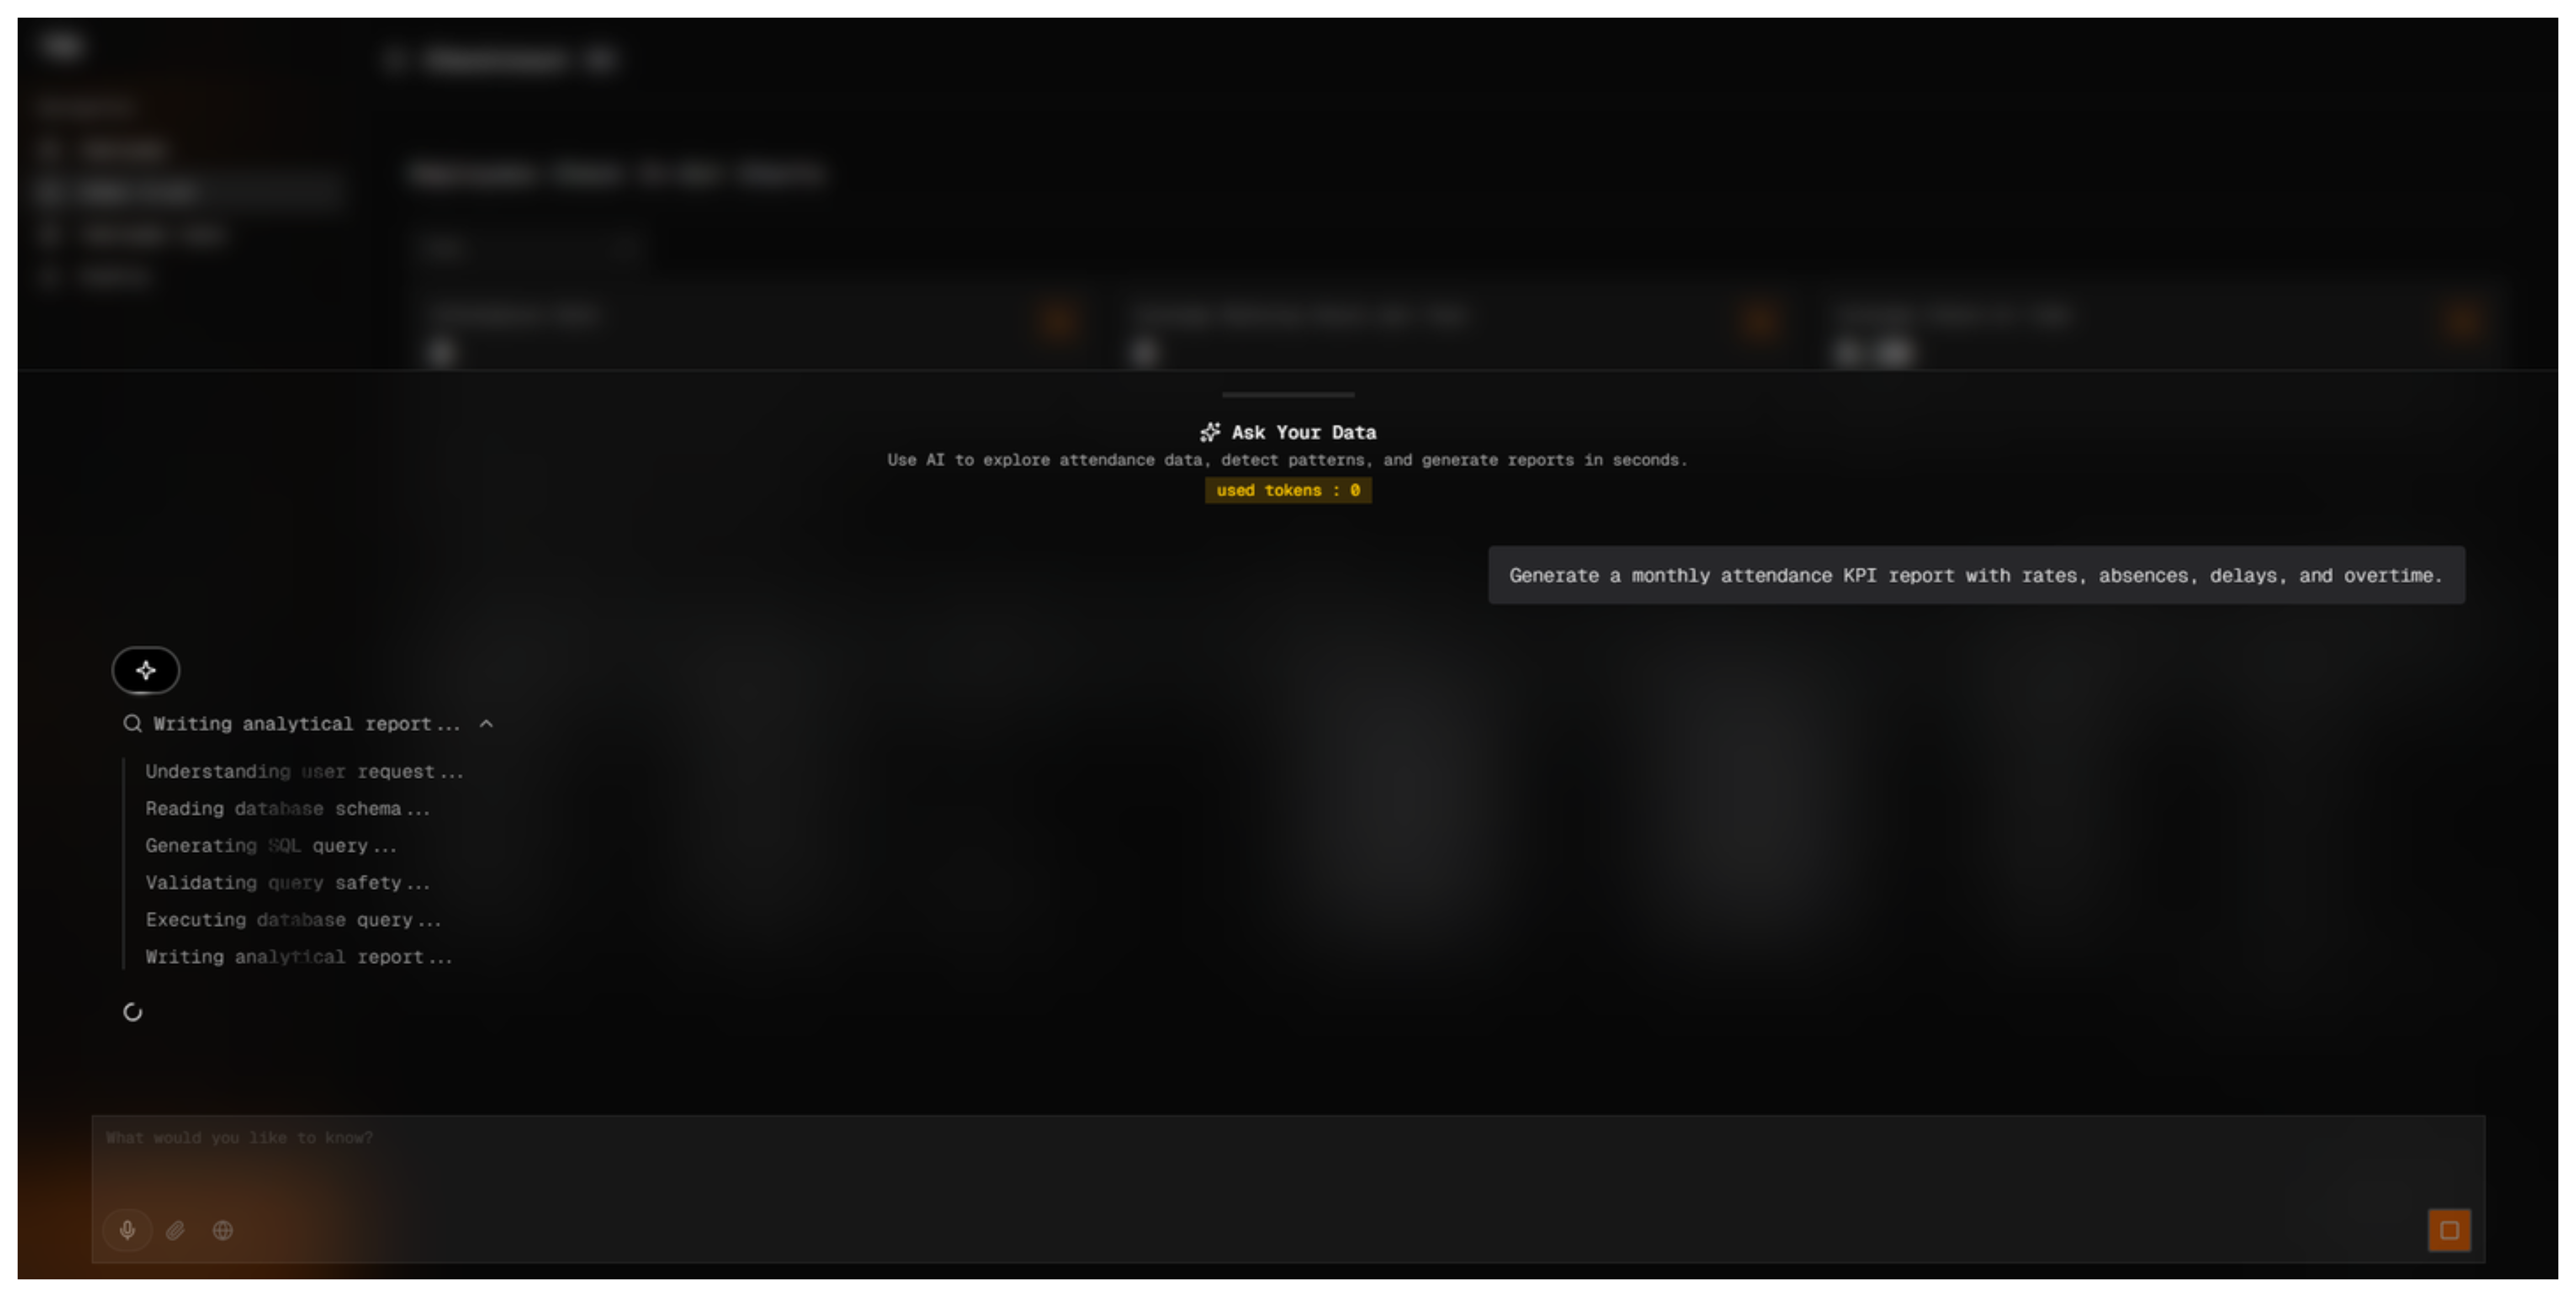
\includegraphics[width=0.92\textwidth,height=0.48\textheight,keepaspectratio]{assets/rh-agent/rh-agent-interface.jpg}
                                                                                                                                    }{%
                                                                                                                                        \fbox{\parbox{0.9\textwidth}{
                                                                                                                                            \centering
                                                                                                                                                \vspace{1.6cm}
                                                                                                                                                    \textit{Missing file: assets/rh-agent/rh-agent-interface.jpg}\\
                                                                                                                                                        \textit{Insert RH Agent interface and interaction screenshot.}
                                                                                                                                                            \vspace{1.6cm}
                                                                                                                                                                }}
                                                                                                                                                                }
                                                                                                                                \caption{RH Agent interface with an example of user interaction}
                                                                                                                                \label{fig:rh-agent-interface}
                                                                                                                                                                \end{figure}


                                                                                                                                                                \section{Conclusion}
                                                                                                                                                                This final stage made the platform more practical to use: users can ask naturally, get guided answers, stream results in real time, and stop generation whenever needed. Overall, the RH Agent improved both usability and operational efficiency.
                                                                                                                                                                